\subsubsubsubsection{Traffic Light}
\begin{figure}[h]
\centering
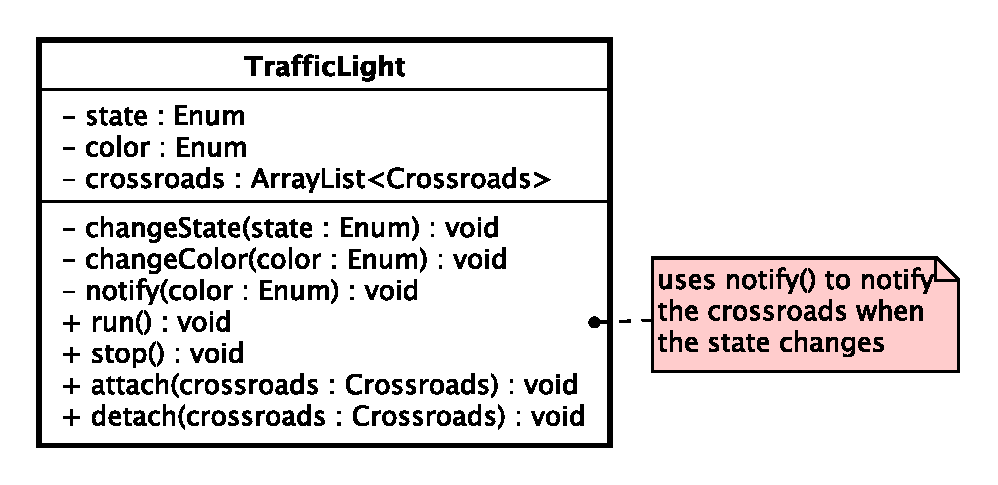
\includegraphics[scale=0.6,keepaspectratio]{images/solution/traffic_light.eps}
\caption{App::Active::TrafficLight}
\label{fig:sd-app-traffic-light}
\end{figure}
\FloatBarrier
\begin{itemize}
  \item \textbf{Description} \\
    It represents an entity that has two possible colors (green, red) and switch
between them after a specified period of time.
  \item \textbf{Attribute}
  \begin{itemize}
    \item \texttt{- state: Enum} \\
The possible states of the entity \{ running, stopped \}.
    \item \texttt{- color: Enum} \\
The possible colors of the entity \{ green, red \}.
  \end{itemize}
  \item \textbf{Operation}
  \begin{itemize} 
    \item \texttt{- changeState(state: Enum)} \\
Change the entity state. This method is used internally by public methods to 
change the entity behaviour.
    \item \texttt{- changeColor(color: Enum)} \\
Change the entity color. This method is used internally by public methods to 
switch between entity colors.
    \item \texttt{+ run(crossroads: Crossroads)} \\
Activates the entity which sets its state to \textit{running}. If its color is 
\textit{green} then it notifies the crossroads and then changes its color, 
otherwise it changes its color to \textit{green} and then notifies 
the crossroad. After changing its color it waits for n seconds.    
    \item \texttt{+ stop()} \\
Stops the entity which sets its state to \textit{stopped}.
  \end{itemize}
\end{itemize}
